\documentclass[tikz]{standalone}
\usepackage{amsmath}
\usepackage{amssymb}
\usepackage{amsfonts}
\usepackage{tikz}
\usetikzlibrary{arrows,decorations.pathmorphing,backgrounds,positioning,fit}
\usetikzlibrary{positioning}

\thispagestyle{empty}
\begin{document}
	\definecolor{nblue}{rgb}{0.40, 0.598, 0.83}
	\definecolor{nred}{rgb}{0.9, 0.65, 0.675} 
	\definecolor{n}{rgb}{0,0,0} % aka black 
	


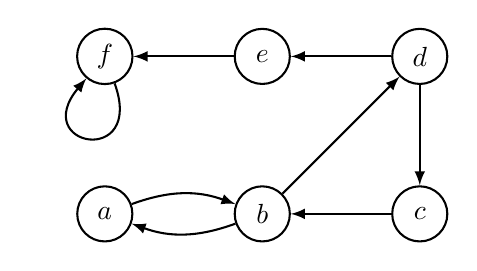
\begin{tikzpicture}[line width=0.75pt, >=latex, minimum size=7mm]

\node[draw, circle] (a) at (0,0) {$a$};
\node[draw, circle] (b) at (2,0) {$b$};
\node[draw, circle] (c) at (4,0) {$c$};
\node[draw, circle] (d) at (4,2) {$d$};
\node[draw, circle] (e) at (2,2) {$e$};
\node[draw, circle] (f) at (0,2) {$f$};
\draw [->] (a) to [out=20,in=160] (b);
\draw [->] (b) to [out=-160,in=-20] (a);
\draw [->] (b) -- (d);
\draw [->] (d) -- (c);
\draw [->] (c) -- (b);
\draw [->] (d) -- (e);
\draw [->] (e) -- (f);
\draw [->] (f) to [out=-70,in=-130,looseness=8] (f);

\end{tikzpicture}

\end{document}

